
\maketitle

\begin{abstract}
Delay embedding parameter selection relies on diagnostics ---
false nearest neighbours, Jacobian-trace convergence, prediction
error --- that implicitly assume deterministic, noise-free
dynamics.  We show empirically that these criteria share a noise
threshold, above which they lose diagnostic value: for the
Lorenz-63 system, false nearest neighbour percentages at the
correct embedding dimension rise from $2\%$ (clean) to $62\%$
($5\%$ noise), while the Jacobian trace becomes uninformative.

We propose residual autocorrelation convergence --- the decrease
of lag-1 autocorrelation in local-linear-fit residuals as
embedding dimension increases --- as a noise-robust alternative.
This criterion correctly identifies sufficient embedding dimension
under $5$--$20\%$ observational noise where deterministic criteria
fail, and provides a U-shaped minimum for lag selection.  Results
are validated on the R\"{o}ssler system.

The computational primitive --- local linear regression in delay
coordinates --- is shared with S-maps~\cite{Sugihara1994} and
Jacobian-based Lyapunov estimation~\cite{SanoSawada1985}.  The
contribution is the application to embedding assessment and the
characterization of noise operating regimes.
\end{abstract}

\begin{quote}\small
\textbf{Keywords.}
delay embedding, embedding dimension, noise robustness, local
linear model, false nearest neighbours, residual diagnostics,
time series analysis.
\end{quote}

% ------------------------------------------------------------------
\section{Introduction}
\label{sec:intro}
% ------------------------------------------------------------------

Delay embedding~\cite{Takens1981, SauerYorkeCasdagli1991}
reconstructs the state space of a dynamical system from a scalar
time series $\{y_t\}$ via delay vectors
\begin{equation}\label{eq:delay}
  \mathbf{z}_t = (y_t,\, y_{t-L},\, \ldots,\, y_{t-(d-1)L})
  \in \mathbb{R}^d.
\end{equation}
The embedding dimension $d$ and lag $L$ must be chosen from data.
Standard criteria include false nearest
neighbours~\cite{KennelBrownAbarbanel1992} (FNN), mutual
information for lag selection~\cite{FraserSwinney1986},
prediction error minimisation~\cite{RagwitzKantz2002}, and
convergence of Lyapunov exponent
estimates~\cite{SanoSawada1985}.

These criteria assume the underlying dynamics are deterministic
and the observations are noise-free.  Under observational noise,
they degrade.  FNN in particular is known to be sensitive to
noise~\cite{RagwitzKantz2002}, but the degradation has not been
systematically characterised.

We characterise the threshold, propose a noise-robust alternative,
and explain why deterministic criteria share the same vulnerability.

% ------------------------------------------------------------------
\section{Method}
\label{sec:method}
% ------------------------------------------------------------------

At each point $\mathbf{z}$ in the reconstructed space, we fit a
local linear model
\begin{equation}\label{eq:local-linear}
  \mathbf{z}_{t+1} \approx A(\mathbf{z})\,
    (\mathbf{z}_t - \mathbf{z}) + \mathbf{b}(\mathbf{z})
\end{equation}
by weighted least squares with a compactly supported tricube
kernel $w(u) = (1 - u^3)^3$ for $\|u\| \leq 1$.  Neighbours
within bandwidth $h$ are identified via KD-tree.  The Jacobian
$A(\mathbf{z}) \in \mathbb{R}^{d \times d}$ is the local
linearisation of the pushforward map.

This computation is shared with S-maps~\cite{Sugihara1994,
DeyleSugihara2011} (used for prediction and causality detection)
and Jacobian-based Lyapunov
estimation~\cite{SanoSawada1985, EckmannKamphorstRuelleEtAl1986}
(used to compute dynamical invariants).  We apply it to a
different question: embedding assessment.

From the local fit we extract two diagnostics:

\medskip
\noindent\textbf{Deterministic diagnostic:} the Jacobian trace
\begin{equation}\label{eq:div}
  \mathrm{div}\, F(\mathbf{z}) = \mathrm{tr}(A(\mathbf{z})),
\end{equation}
averaged over the attractor.  For a faithful embedding of a
deterministic system, $\langle\mathrm{tr}(A)\rangle$ converges
to the sum of local Lyapunov exponents as $d$ increases.
Instability of $\langle\mathrm{tr}(A)\rangle$ with $d$ indicates
insufficient embedding.

\medskip
\noindent\textbf{Residual diagnostic:} the lag-1 autocorrelation
of residuals
\begin{equation}\label{eq:residual}
  \varepsilon_t = \mathbf{z}_{t+1} -
    \bigl(A(\mathbf{z}_t)\,(\mathbf{z}_t - \mathbf{z}_{\mathrm{nn}})
    + \mathbf{b}(\mathbf{z}_{\mathrm{nn}})\bigr),
\end{equation}
where $\mathbf{z}_{\mathrm{nn}}$ is the nearest query point.  If
the embedding is sufficient and the local linear model captures the
deterministic dynamics, $\{\varepsilon_t\}$ should be white noise.
Remaining autocorrelation indicates deterministic structure not
captured by the embedding.

The criterion: \emph{the embedding dimension is sufficient when
the residual lag-1 autocorrelation stabilises near zero.}  For lag
selection: \emph{the optimal lag minimises the residual
autocorrelation at sufficient $d$.}

% ------------------------------------------------------------------
\section{Noise threshold for deterministic criteria}
\label{sec:threshold}
% ------------------------------------------------------------------

Both diagnostics of~\S\ref{sec:method} require a local linear fit,
which in turn requires neighbours within bandwidth $h$.  We test
on Lorenz-63 ($N = 50\,000$, $\Delta t = 0.01$, $h = 5$, $L = 10$),
observing the $x$-component corrupted by additive Gaussian noise
at amplitudes $0$--$20\%$ of the signal standard deviation.

Table~\ref{tab:fnn} shows FNN percentages (threshold $R = 2$) at
the correct embedding dimension $d = 3$ as a function of noise
level.

\begin{table}[h]
\centering
\begin{tabular}{@{}lcccccc@{}}
\toprule
Noise (\%) & 0 & 1 & 2 & 5 & 10 & 20 \\
\midrule
FNN at $d = 3$ (\%) & 1.8 & 27.0 & 40.6 & 62.4 & 74.5 & 79.4 \\
\bottomrule
\end{tabular}
\caption{False nearest neighbour percentage at the correct embedding
dimension $d = 3$ for the Lorenz-63 system under varying
observational noise.  Above $\sim 2\%$ noise, FNN incorrectly
rejects the true dimension.}
\label{tab:fnn}
\end{table}

The mean $|\langle\mathrm{tr}(A)\rangle|$ across the attractor
shows a similar threshold.  For clean data, it increases from
$0.7$ ($d = 2$) to $47.7$ ($d = 6$), clearly indicating
dimension convergence.  At $5\%$ noise, the range collapses to
$0.02$--$0.68$: no diagnostic signal remains.

The transition is sharp: at $2\%$ noise, diagnostic signal
persists (range $0.7$--$7.2$); at $5\%$, it vanishes.
Figure~\ref{fig:phase} shows the full noise--dimension phase
diagram for both diagnostics.

\begin{figure}[t]
\centering
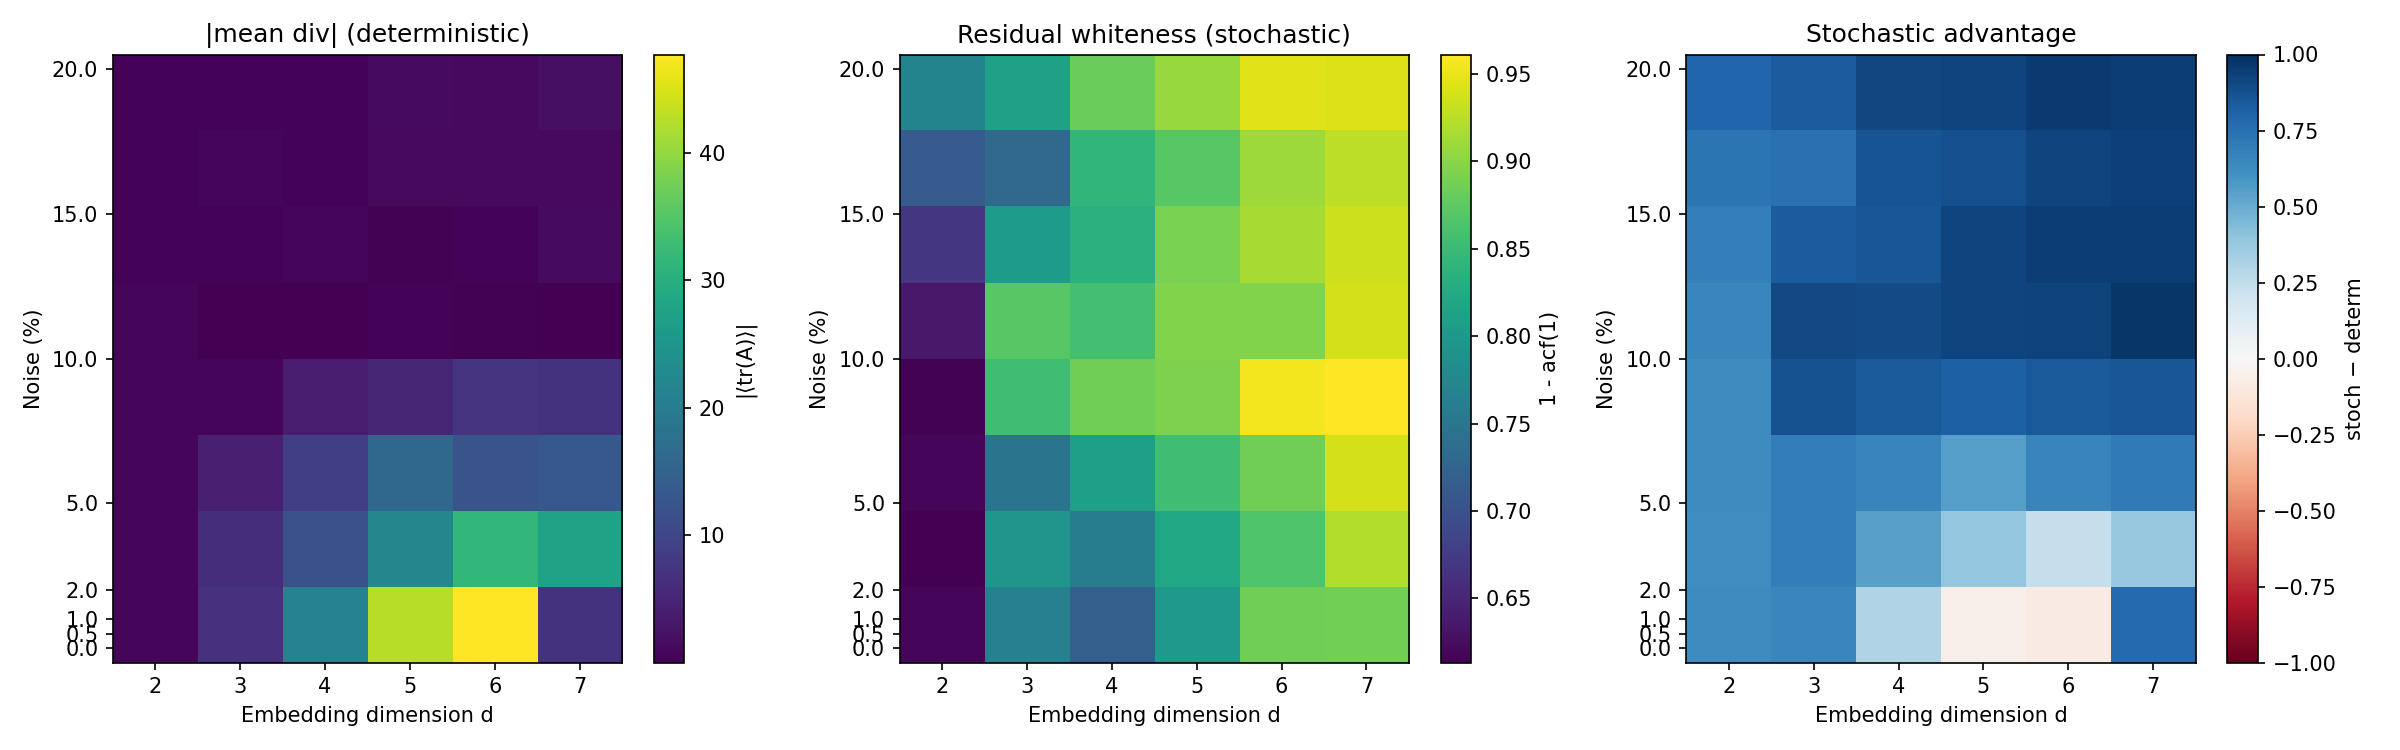
\includegraphics[width=\textwidth]{code/phase_diagram.png}
\caption{Phase diagram: noise level vs.\ embedding dimension for
the deterministic diagnostic (left: $|\langle\mathrm{tr}(A)\rangle|$)
and the residual diagnostic (centre: $1 - \mathrm{acf}(1)$,
where higher = whiter residuals).  The deterministic diagnostic
loses signal above $\sim 2$--$5\%$ noise; the residual diagnostic
functions across the full range.}
\label{fig:phase}
\end{figure}

% ------------------------------------------------------------------
\section{Residual autocorrelation as embedding criterion}
\label{sec:residual}
% ------------------------------------------------------------------

The Jacobian trace fails above $\sim 2\%$ noise because it tests a
property (well-defined local expansion rate) that noise destroys.
The residual diagnostic tests a different property: absence of
predictable structure in the fit errors.

Table~\ref{tab:acf} shows the lag-1 residual autocorrelation as a
function of embedding dimension, for both clean and $5\%$-noisy
Lorenz data.

\begin{table}[h]
\centering
\begin{tabular}{@{}lcccccc@{}}
\toprule
$d$ & 2 & 3 & 4 & 5 & 6 & 7 \\
\midrule
Clean: acf(1) & 0.38 & 0.24 & 0.28 & 0.20 & 0.11 & 0.11 \\
Noisy (5\%): acf(1) & 0.36 & 0.13 & 0.14 & 0.11 & 0.11 & 0.06 \\
\bottomrule
\end{tabular}
\caption{Lag-1 residual autocorrelation versus embedding dimension.
Both clean and noisy data show a decreasing trend, stabilising at
$d \approx 5$--$6$.  The criterion works under noise where FNN and
Jacobian trace do not.}
\label{tab:acf}
\end{table}

\noindent The residual autocorrelation decreases with $d$ and
stabilises across the full noise range tested ($0$--$20\%$).

At fixed $d = 3$, the residual autocorrelation as a function of
lag $L$ shows a U-shaped profile with a minimum near $L \approx
7$--$11$ (corresponding to $0.07$--$0.11$ orbital periods).  This
minimum persists under $5\%$ noise (Figure~\ref{fig:lag}),
providing a noise-robust lag selection criterion.

\begin{figure}[t]
\centering
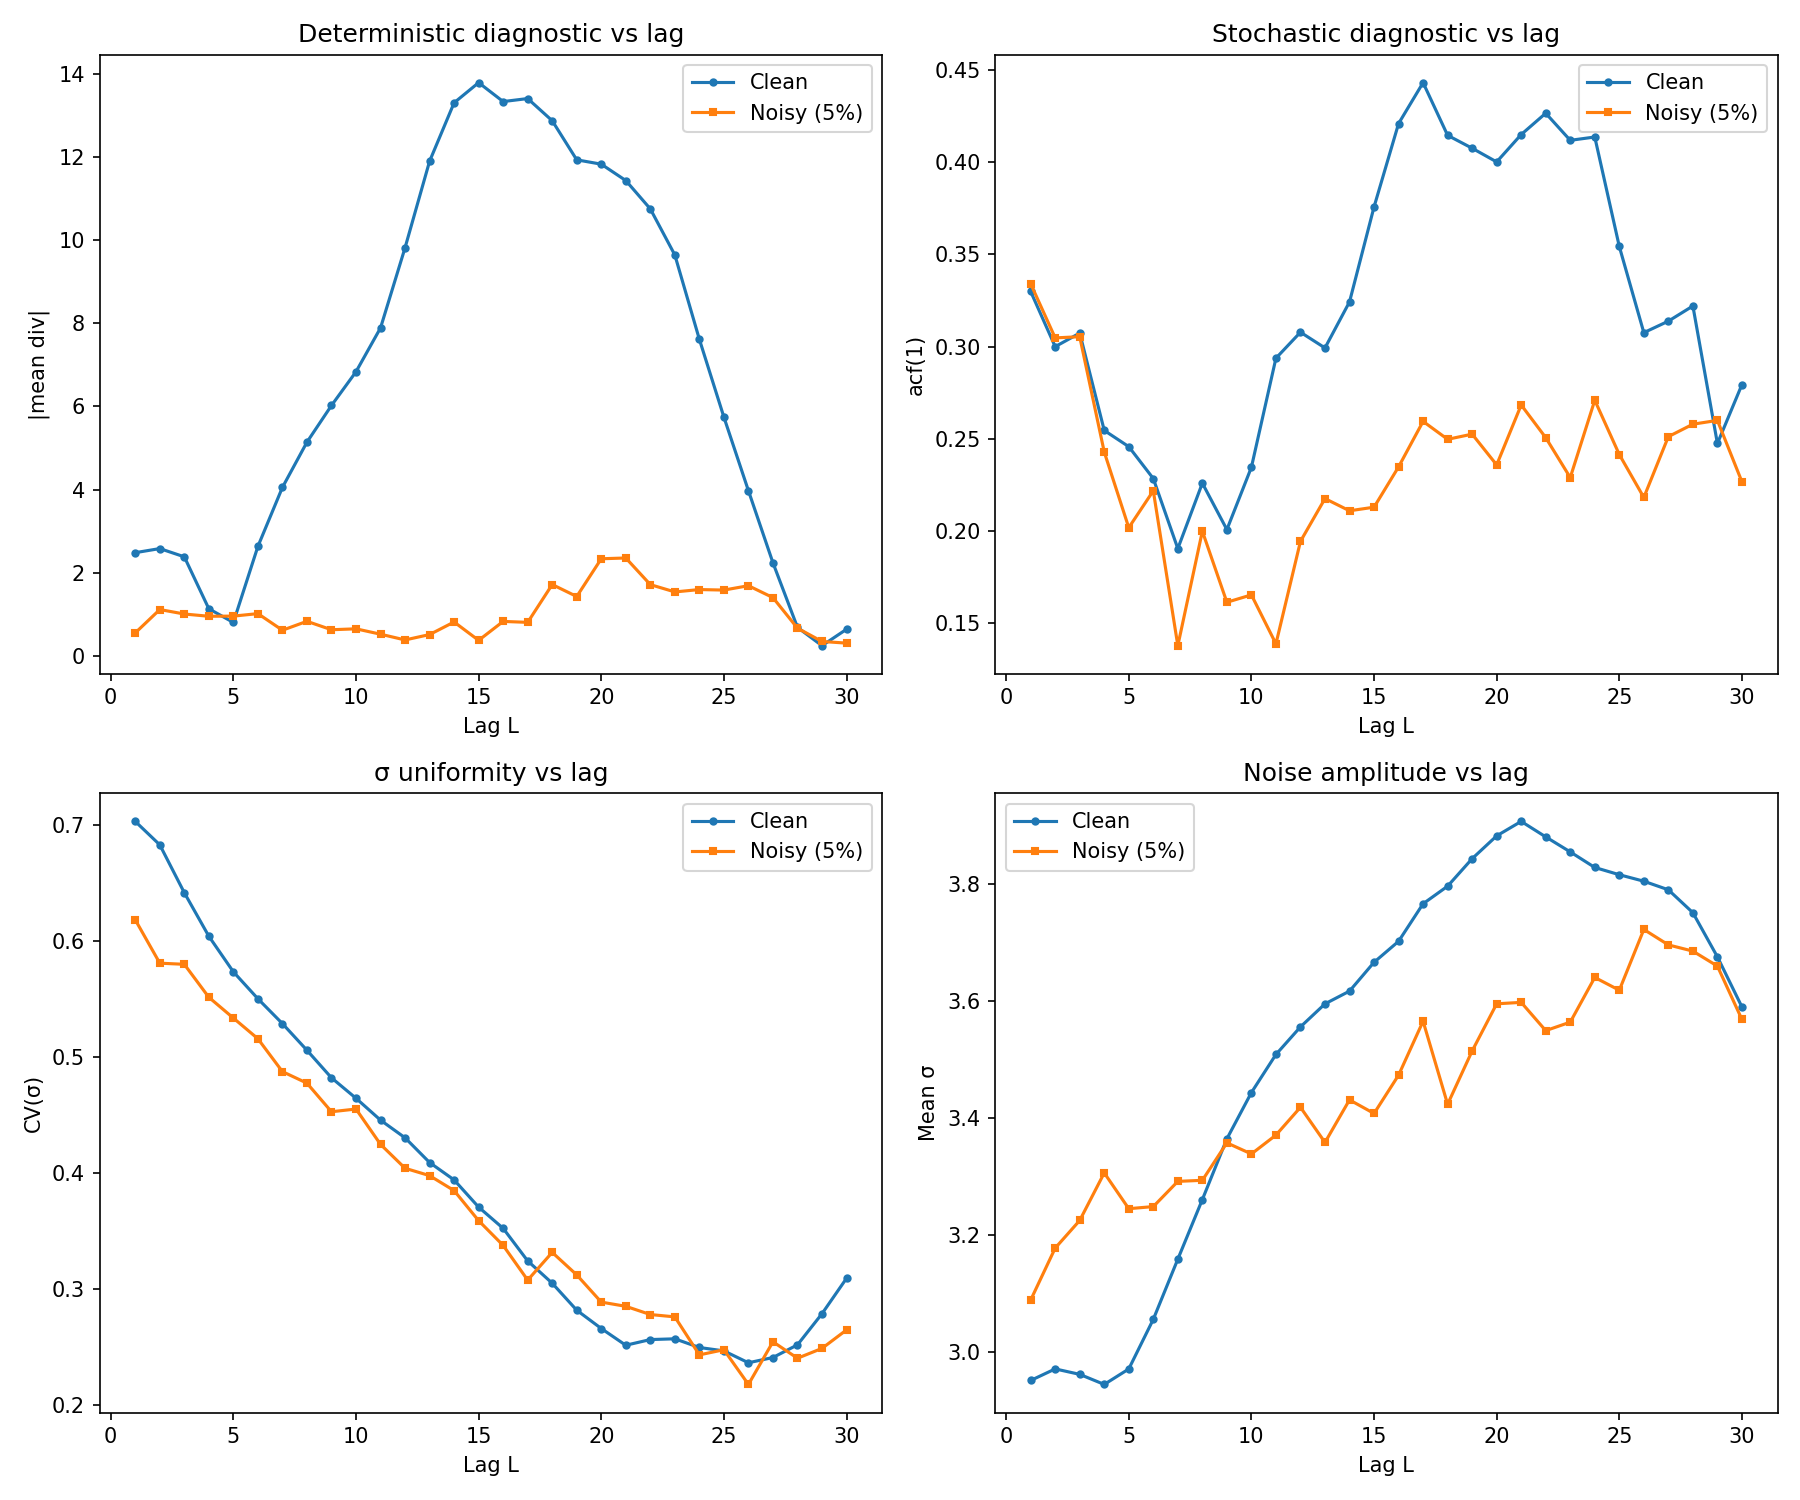
\includegraphics[width=0.8\textwidth]{code/lag_sweep.png}
\caption{Lag sweep ($d = 3$, Lorenz-63).  Top left: Jacobian
trace vs.\ lag (bell-shaped for clean, flat for noisy).  Top
right: residual acf(1) vs.\ lag (U-shaped for both clean and
noisy, minimum at $L \approx 7$--$11$).}
\label{fig:lag}
\end{figure}

The same patterns hold for the R\"{o}ssler system ($a = 0.2$, $b =
0.2$, $c = 5.7$): residual autocorrelation decreases with $d$ for
both clean (0.14 $\to$ 0.03) and noisy data (0.09 $\to$ 0.01),
while the Jacobian trace diagnostic works only for clean data.

% ------------------------------------------------------------------
\section{Discussion}
\label{sec:discussion}
% ------------------------------------------------------------------

The shared noise vulnerability of FNN, Jacobian trace, and
Lyapunov convergence is not coincidental.  All three test for
properties of deterministic dynamics: FNN tests for injectivity of
the delay map; the Jacobian trace tests for well-defined local
expansion rates; Lyapunov convergence tests for stability of
dynamical invariants.  Observational noise destroys injectivity
(nearby points in delay space may be far apart in state space due
to noise), corrupts Jacobian estimates, and introduces spurious
Lyapunov exponents.

The residual criterion survives because it tests a different
property: whether the local linear model has captured all
\emph{predictable} structure, regardless of noise.  Residual
autocorrelation measures remaining deterministic signal in the
prediction errors --- a property that is well-defined even when
the dynamics are stochastic.  The embedding is sufficient when no
deterministic structure remains in the residuals.

This distinction corresponds to a difference in modelling
commitment.  Deterministic criteria implicitly assume $\mathbf{z}_{t+1}
= F(\mathbf{z}_t)$ (single-valued dynamics); noise violates this
assumption and the criteria respond to the violation rather than
to embedding insufficiency.  The residual criterion assumes
$\mathbf{z}_{t+1} = F(\mathbf{z}_t) + \sigma(\mathbf{z}_t)
\boldsymbol{\eta}_t$ (drift plus diffusion); noise is built into
the model, and the diagnostic tests only for remaining
deterministic structure.

The embedding problem is algebraically underdetermined: the
observation algebra determines a measure on compatible
observation-patterns but does not constrain which patterns
correspond to realised states~\cite{mahon2026}.  This is why
embedding selection is necessarily empirical, and why different
empirical criteria have different operating regimes.  The practical
recommendation: for clean data ($< 2\%$ noise), deterministic
criteria (FNN, Jacobian convergence) provide sharp diagnostics.
Above this threshold, use residual autocorrelation convergence for
dimension selection and the U-shaped minimum for lag selection.

The local linear computation is shared with
S-maps~\cite{Sugihara1994, DeyleSugihara2011, CenciSugiharaSaavedra2019}
(prediction and causality) and Ragwitz--Kantz~\cite{RagwitzKantz2002}
(embedding selection via prediction error).  Ragwitz--Kantz
minimise out-of-sample prediction error over $(d, L)$, which is
prediction-optimised; our residual autocorrelation criterion is
sufficiency-based.  These can disagree: prediction skill may
plateau before residuals whiten (diagnostic underfitting) or
overfit in noisy regimes.

Cenci et al.~\cite{CenciSugiharaSaavedra2019} regularise S-maps
under noise; regularisation of the local Jacobian may extend the
operating regime of the deterministic diagnostic, but this is not
explored here.

\subsection*{Limitations}

The noise threshold ($\sim 2$--$5\%$) is characterised empirically
for two systems (Lorenz-63, R\"{o}ssler).  Its dependence on
attractor dimension, data length, and bandwidth is not
systematically explored.  The residual criterion requires
sufficient data to estimate local linear maps reliably; in very
high dimensions or with sparse data, both criteria may fail.

\bibliographystyle{plain}
\bibliography{references}
